\chapter{Grundlagen}

Dieses Kapitel gibt eine  

% AR, Traking Methoden, Situative Visualisierung, Kommunikation, Usability Usability Engenieering als Methode,Open Innovation 

\section{Augmented Reality}

%Definition und Begriffseingrenzung  von AR
Abzugrenzen von VR  ist Augmented Reality (AR). [SchmalstiegHöllerer16] Im Gegensatz zu virtuellen Realität wo Benutzer vollständig in virtuelle Umgebungen eintauchen,
ist das Ziel von AR, Informationen direkt in die physiche Ubgebung des Benutzers einzufügen. So soll der Eindruck erweckt werden, dass diese Informationen Teil der wirklichen Welt sind. % Als Fußnote anmerken: Informationen müssen hierbei nicht nur auf visuelle Informationen beschränkt sein, sondern es kann sich dabei auch um auditive, haptische, gustative oder auch olfaktorisch Informationen sein.
[Azuma 1997] Während in VR, Benutzer von der Äußeren Umgebung nichts mitbekommen, wird mit AR Systeme die wirkliche Umebung des Benutzers, mit vitruellen Objekten überlagert. 
Azuma beschreibt folgende Charakteristiken für AR Systeme: 

\begin{enumerate}
	\item Kombinieren Digitale und Reale Welt.
	\item Ermöglichen Interaktionen in Echtzeit.
	\item Informationen haben einen Bezug zum 3D Raum.
\end{enumerate}

Diese Characteristiken helfen dabei den Begriff Augmented Reality besser einzugrenzen zu können. [Azuma97 ] Filme wie z. Bsp.  ``Jurassic Park`` in welchen virtuelle Objekte in die reale 3D Szene eingefügt werden, 
erwecken den Eindruk dass diese Objekte Teil der realen Szene sind, jedoch kann mit diesen Objekten nicht in Echtzeit interagiert werden. [Tönnis2010] In Filmen werden die virtuellen Objekte in eine zuvor augezeichnete 
Aufnahme eingefügt. In AR werden diese in ein live Video eingefügt. In Filmen steht für das Einfügen von digitalen Informationen in die reale Szene eine viel größere Zeit zur Verfügung. In AR muss dies in einer Zeit kleiner 
als 

Ein anderes Beispiel ist im Vorschaufenster von Digitalkameras zu sehen. Oft blenden Digitalkameras im Vorschaubild, Informationen zum Ladezustand der Batterie, Aktivierung des Bilitzes und weitere 
Informationen bezüglich den aktuellen Einstellungen. Diese Informationen überlagern zwar die realen Objekte in der Szene, haben jedoch keinen Bezug zu den im 3D Raum befindenden Objekte. 
Der elektronishe Sucher hingegen welches Objekte (z. Bsp. Gesichter) erkennt und in einem virtuellen Rahmen einrahmt, hat ein Bezug zu den Objekten im 3D Raum. Zudem sind Interaktionen in Echtzeit möglich.  
Bewegt sich das vom virtuellen Rahmen,  eingerahmte reale Objekt, oder die Kamera selbst, verändert sich auch die Position des virtuellen Rahmens. 

\begin{figure}[H]
	\centering
	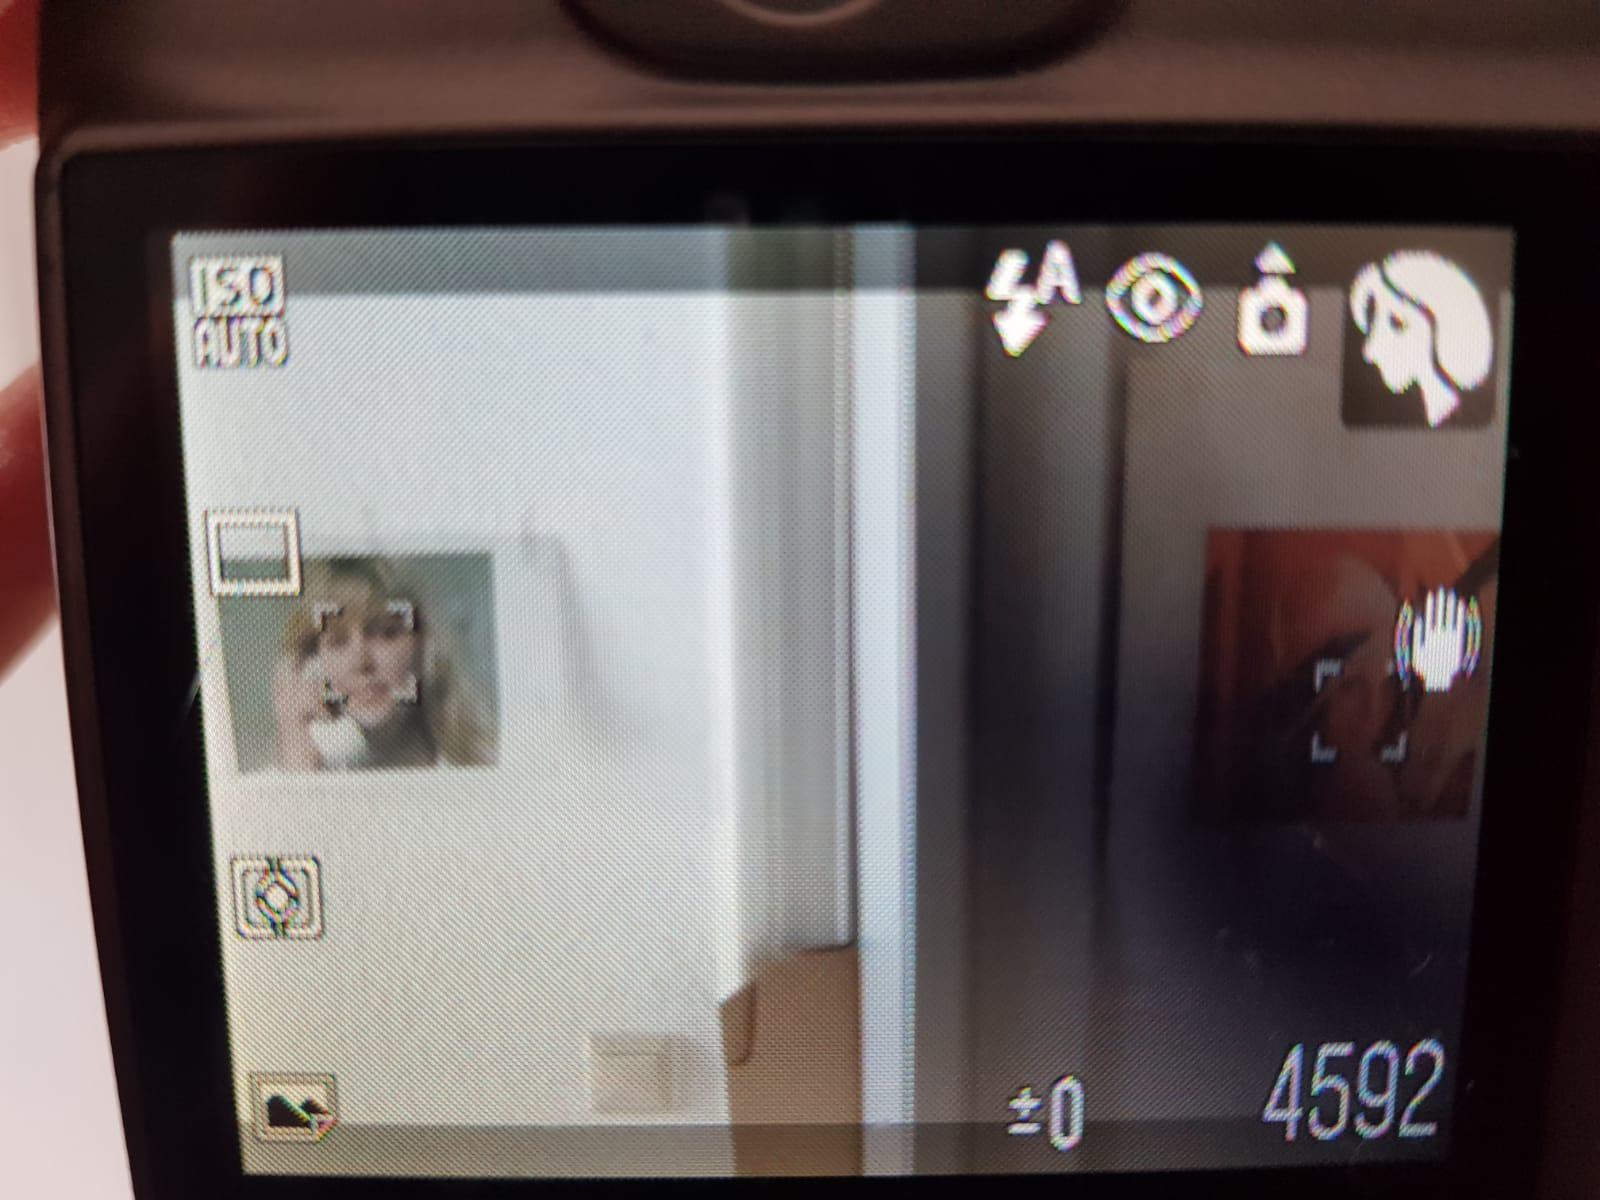
\includegraphics[width=0.95\textwidth]{resources/fundamentals/example_camera_screen_ar}
	\caption{Beispiel CNN Arhcitektur \cite{typical_cnn_img}}
	\label{img:cnn_example_network}
\end{figure}

% Motivation
[Azuma97] Durch das kombinieren von vitueller und physischer Welt, erweitert Augumented Reality die Wahrnehmung des Menschen. Die Motivation von AR ist, den Menschen durch das Einfügen
von digitaler Informationen in die physische Welt, Hinweise zu geben und Details zu zeigen die er mit seinen Sinnen sonst nicht unmittelbar wahnehmen könnte. Die Informationen sollen den Menschen 
bei der Verrichtung ihrer Aufgaben in der physischen Welt unterstützen.

% Anwendungsfelder von AR % Besonders passend für diese Arbeit sind Annotationen und Warung und Reperatur. Da diese sich besonders mit Interaktionen an Realen Objekten, meist Produkte befassen.
Azuma fasst in [Azuma97]  Forschungen zu AR in sechs Anwendungsgebiete zusammen. Zur Visualisierung von Medizindaten, in der Wartung 
und Instandsetzung, Annotationen, für die Wegfindung für Roboter und für die Navigation von Militärflugzeugen. Beispielsweise können Annotatinen 
verwendet werden um Informationen über den Inhalt von Regalen einzublenden während ein Nutzer durch ein Bibliothek läuft. % Füge hier vielleicht noch ein Beispiel dazu ein % Füge hier Verweis auf ein Artike als Fußnotel hinzu
Auch können Annotationen in AR verwendet werden um einzelne Bauelemente an komplexen Bauteiteilen zu identifizieren und Informationen über diese zu anzuzeigen. 
In der Wartung und Instandsetzung können Augemented Reality Anwendungen dabei helfen Instruktionen an komplexen Maschinen und Anlagen zu visualisieren welche sonst in 
Form von Text und Bildern vorliegen. So können virtuelle Replikate über die physischen Modelle gelegt, und so Schritt für Schritt Anleitungen direkt am physichen Produkt angezeigt werden. 
Durch Animationen können diese Anleitungen mit präziser gestaltet werden und zum Beispiel auch Informatinen über die Richtung geben. 

Diese Systeme können heute zum Beispiel Unternternehmen dabei helfen besser mit ihren Kunden zu kooparieren. In Kombination mit der Technologie Internet of Things (IOT)  können Unternehmen,
zustandsbezogene Informationen zu Ihren Systemen bei Endkunden abrufen und proaktiv Ihre Kunden auf notwendige Wartungen aufmerksam zu machen. Wartungsanleitungen können dann direkt 
an den Analgen angezeigt werden.%TODO mach Verweis für Wartung (z. Bsp:https://www.ptc.com/-/media/Files/PDFs/Case-Studies/Howden-vuforia-studio-case-study-Feb-2019.pdf?la=en&hash=6342841E1B6470C1F313295427398606)

%Grundlegende Techniken
% file:///C:/Users/alibe/Desktop/papers/MarcusTönnis_einblicke_in_augmented_reality.pdf Seite 32
[Tönnis2010] Für die Überlagerung der realen Welt mit virtuellen Objekten eignen sich aktuell zwei Display Techniken,  Optical See-Through und Video See-Through. 
Bei Optical See-Through kann der Nutzer direkt in die reale Welt blicken und computer generierte Bilder werden auf ein halbdurchlässiges Spiegel eingeblendet (dieses wird als Combiner bezeichnet).
Diese Technik hat den Vorteil dass der Nutzer einen direkten Blick auf die reale Welt hat. Der Nachteil ist jedoch dass die reale Welt nicht zeitgleich mit virtuellen Objekten überlagert werden kann. 
Dadurch dass die Berechnung für die Positionsbestimmung und das Rendern der virtuellen Objekte Zeit in Anspruch nimmt, werden diese mit einer kleinen Verzögerung angezeigt. Dies kann auch 
wenn es nur sich nur um einige Milisekunden handelt zu einem so genannten Schwimmefekt führen (en. lag). Mit der See Through Display Technik, wird die reale Welt dem Nutzer als ein Video 
gezeigt und mit virtuellen Objekten überlagert. Der Vorteil dieser Technik liegt darin, dass die Darstellung der realen Welt um die Zeit verzögert werden kann die benötigt wird um die virtuellen Objekte 
richtig zu positionieren und rendern. Dadurch werden die Nachteile der Optical-See-Through Technik kompensiert. Dass die reale Welt dem Nutzer verzögert angezeigt wird bringt jedoch den Nachteil 
dass Positionsänderunen von physischen im realen Welt befindenden Objekten oder die Änderung der Perspektive falls sich der Nutzer selbst bewegt verhzögert angezeigt wird. Zudem wird mit 
dieser Technik je nach Auflösung der Kamera die reale Welt mit verringerter Qualität angezeigt. [SchmalstiegHöllerer16 Seite 368] Vor allem bei der Kommunikation mit anderen Personen können diese 
Nachteile zu Problemen führen. 

\section{Objekterkennung und- Verfolgung}

% Definition von Objekterkennung und Verfolgung

% Geschichte und Entwicklung

\subsection{Markerbasiertes Tracking}

% Begriffserklärung von Marker Trakting

% Anwendungsfelder von Marker Traking

\subsection{Markerloses Tracking}

% Begriffserklärung von Markerlosen Traking 

% Anwendungsfelder von Markerlosen Traking

\section{Situated Visualization}

Das zu konzipierende System sollte durch den Einsatz von Augmented Reality Rückemeldungen zum Design von Produkten und das explorieren dieser Rückemeldungen ermöglichen. Damit dies gut gelingt 
ist ein gutes Verständnis von Situated Visualization und teilweise auch von Situated Analytics notwendig. 

[SchmalstiegHöllerer16 Seite 239] Ein großer Vorteil von Augmented und Mixed Reality Nutzeroberflächen ist,  dessen Fähigkeit, situationsrelevante Informationen bezüglich einer Aufgabe oder Anwender anzeigen zu können. 
Es ist jedoch nicht sehr davon abhängig welche Informationen in welcher Form in AR angezeigt werden um diesen Voreil von AR ausschöpfen zu können. Situated Visualization befasst sich damit wie Computer generierte Grafiken 
in die reale Szene eingefügt und angemessen presäntiert werden. 


https://link.springer.com/content/pdf/10.1007%2F978-3-030-01388-2.pdf
refers to data representations that are related to and portrayed in their physical environment. Sensemaking is achieved through the combination of the visualization and the relationship of that visualization to the immediate physical environment
% Embedded Visualizations seite 205 (Seite 210 ist sehr interessant. Beispiel mit SterilAnzug und Nutzerfeedback).  Seite 220 embedded vs. situated.

\begin{table}[htbp]
\caption{Situatedness vs. Analytic Level}
	\begin{center}
		\begin{tabular}{|l|ll|}
		\hline
		\textbf{Situatedness}& \textbf{Analytic Level Low} & \textbf{Analytic Level High}\\
		\hline
		\textbf{High } & Situation Awareness & Situated Analytics \\
		\textbf{Low} & Information Displays/ Ambient Displays & Visual Analytics/ Traditional Analytics \\
		\hline
		\end{tabular}
	\end{center}
	\label{tab:categorycscw}
\end{table}


% welche Informationen? % The power of AR as a novel user interfae paradigm derives in large part from its ablity to display information that is relaevant to a situation, task or user. 
%To sucessfully comunicate the desired information, it must be put in an appropriate visual form. This is done through the application of suitable visualizwation techniques. 

% Information seeking mantra nach Shneiderman

% Falls die die Informationsmenge zu groß oder zu Komplex wird beschreiben Daniel A. Keim et. al: visual analytics mantra
%Neven A. M. ElSayed et. all %  Situated Analytics has four primary elements: situated information, abstract information, augmented reality interaction, and analytical interaction

%Herrausforderungen: Unordnung duruch zu viele Daten (Überlagerung). Generell auch bei anderen visualisierungen. Durch limitierter Platz bei AR manchmal besonders verschlimmert. %Registrierungsfehler führen zur falschen platzierung von visualisierungen. 
% Störende\ Ungünstige Visualisierung. Auch wenn Registrierung theoretisch ganz fehlerfrei funtionieren würde, ungünstig sein und die Fähigkeit des Nutzers wichtige Informationen von nicht relevanten Informationen. 

% In folgendem werden Techniken für die Bewältigung dieser Herrausforderungen vorgestellt. 

Data Overlay 

% la

% Labeling und Annotationen


% 


\section{Computerunterstützte Kollaboration}

% Ziel des zu entwickelnden Systems, ist die erfolgreiche Kommunikation von Design Ideen durch den Endkunden. Kommunikation erfordert Kollaboration von Teilnehmern? Kunde <-> Kunde, Kunde <-> Hersteller zum Beispiel.  %Dazu schauen wir uns die computergestützte Collaboration näher an.

[SchmalstiegHöllerer16 Seite 362] In der computerunterstützten kooperativen Arbeit (en. Computer-supported cooperative work (CSCW)) ist eine Karegorisierung in Synchrone oder Asychrone und Co-located oder Remome sehr verbreitet. 
Hierbei wird nach der zeitlichen (Synchron/ Asynchron) und nach der räumlichen (Co-located/ Remote ) Dimension der Kommunikation unterschieden. Betrachtet man die zeitliche Dimension, können mehrere Nutzer zur gleichen Zeit miteinander kommunizieren
oder aber zur unterschiedlicher Zeit (also unabhäting voneinander) kommunizieren. In der räumlichen Dimension können Nutzer entweder am gleichen Ort miteinander kommunizieren oder entfernt voneinander sein. 

\begin{table}[htbp]
\caption{Kategorisierung Computer unterstützter Cooperationssysteme in Bezug zu AR}
	\begin{center}
		\begin{tabular}{|l|ll|}
		\hline
		 & \textbf{Co-located} & \textbf{Remote}\\
		\hline
		\textbf{Synchronous} &  AR shared space & AR telepresence \\
		\textbf{Asynchronus} & AR annotating/ browsing (in-situ) & Generic sharing\\
		\hline
		\end{tabular}
	\end{center}
	\label{tab:categorycscw}
\end{table}

AR annotation\ browsing (in-situ). % laut Schmalstig ung Höllerer welche dieses Model von Rodden,  im Kontext von AR Anwendungen beschreiben, vergleichbar wie Graffitti.  

[Rodden seite 20]
% [Rodden seite 24] Co-authoring systems aim to support some of the most fundamental parts of cooperation by supporting the negotiation processes % for commenting %multiple users working on % [Rodden seite 24]store and forward and real-time communication systems. %notwendigkeit für unterscheidung zwischen private, public oder direkte nachrichten 
The general model adopted by these systems is that of asynchronous co-operation with each user working independently on a portion of the document. Reviews and comments are added to the document by annotating sections of the document. 

[SchmalstiegHöllerer16 Seite 362] Asychronous AR is less frequently utilized. The most important use case in this category is the annotation of a physical environment by one user and later in situ browsing or editing of the annotations by another user.
You might think of this application as a sort of virtual graffiti. 


% Immersive analytics seite 239

However, distributed asynchronous collaboration involves capturing input from people at different times and different placesandsocanprovidesomeuniquebenefits.Forexample,Benbunan-Fichet al. found that asynchronous collaboration can produce broader discussions and more complete reports from group discussions than their face-to-face counterparts [9]. Other benefits include enabling people to contribute whenever they have time to provide input [104], they can work on the part of the problem that they feel most qualified to address [129], and can combine information from a variety of sources [52].


\section{Usability}

% Ziel der Arbeit ist ein Weg zu finden um effektiv und effizient Produktdesignbeschreibungen an Produkten zu zeigen mit einsatz von Augmented Realiy und verschiedene Techniken zu 
%vergleichen. Dafür muss ein besonderer Fokus auf die Usablity gelegt werden. Daher hier usability...
Einen besonderen Fokus soll diese Arbeit auf die Usability legen. Daher wird in folgendem Abschnitt die Begriffsdefinition von Usablity näher beleuchtet, es werden einige 
gängige Methoden für die nutzerzentrierte Gestaltung und Entwicklung von Systemen vorgestellt und abschließend Methden für Usability Tests und Evaluirung erleutert. 

\subsection{Was ist Usability?}

% Begiffserklärung von Usability
In der Normreihe ISO 9241 welches als ein internationaler Standard, Richtlinien für die Gestaltung von Mensch-Computer-Interaktionen beschreibt, wird im ISO Norm 9241-11,  Usability wie folgt definiert:

"das Ausmaß, in dem ein Produkt durch bestimmte Benutzer in einem bestimmten Nutzungskontext genutzt werden kann um bestimmte Ziele effektiv, effizient und zufriedenstellend zu erreichen."

% Usablity nicht nur Gestaltung der Nutzeroberfläche
[MichaelRichterMarkusFlückiger16; MaryBethRosson02] Usablity wird  oft als ein Qualitätskritärium für die Gestaltung der Benutzerschnittstelle verstanden. Dies ist jeodoch nicht ganz richtig.

%Die Benutzbarkeit eines Systems muss im Kontext seiner Verwendung beurteilt werden.[Michael Richter, Markus Flückiger]
Dass die Usability eines Systems nach dessen Nuzungskontext zu beurteilen ist verdeutlichen Michael Richter und Markus Flückiger an einem konkreten Beispiel für die Erfassung 
von Kurznachrichten (SMS) mit dem Aufkommen von Mobiltelefonen.  Bevor Smartphones mit Touchdisplays verbreitet waren, hatten Mobiltelefone oft rein numerische Tastaturen sodass, das Erfassen 
von Textnachrichten über die Nutzung der numerischen Tasten erfolgen musste. Indem zum Beispiel in kurzen Zeitabständen zwei mal auf die Taste "2" gedrückt wurde, wurde zu Beispiel der Buchstabe ``B`` eingegeben. 
Diese Eingabemethode wurde oftmals von vielen Nutzern als umständlich empfunden. Jedoch konnte auf diese Weise effizient und zufridenstellend die die Aufgabe, eine Kurznachricht zu erfassen erfüllt werden. 
Zudem war diese Methode einfach zu erlernen und einprägsam. Somit wies diese Methode eine hohe Usablity auf. 

% Usablity nicht nur User friendly
[Nielsen94; Rex HartsonPardhaSPyla12] Oft wird Usablity auf die Eigenschaft eines Systems reduziert besonders benutzerfreundlich (en. User- friendly) zu sein. Der Begriff Usabliy umfasst jedoch mehr Aspekte. 

[Nielsen94] Mit dem Begriff "User- friendly" als Synonym für Usablity würde impliziert werden dass die Bedürfnisse von Benutzern mit nur einer einzigen Eigenschaft eines Systems beschrieben werden kann. 
In der Realität haben jedoch unterschiedliche Nutzer, unterschiedliche Bedürfnisse. Ein System welches zu einem Nutzer freundlich erscheint, könnte unter Umständen von einem anderen Nutzer als lästig empfunden werden.

% Eine Teilmenge der Systemazeptanz 
Nielsen Unterteilt Akzeptanzkriterien für ein Systems in soziale und praktische Kriterien.

Soziale bzw. ethische Akzeptanzkriterien sind solche, welche  die Nutzer von der Nutzung eines Sytems abhalten, selbst wenn praktische Akzeptanzkriterien sehr gut erfült werden. 
Spiekermann [vgl. Spiekermann 2016: 285] führt hierzu ein gutes Beispiel für ein solches Kriterium auf. Sie beschreibt am Beispiel eines Körperscanners an Flughäfen, dass trotzt  Berücksichtigung vieler 
praktischer Aspekte wie Ergonomie und trotz der effizienten und effektiven Aufgabenerfüllung ein solches System wenig Akzeptanz von den Nutzern haben kann. Beisielsweise fühlten sich Passagiere 
unangenehm wenn der Bildshirm auf welchem die nackten Umrisse ihrer Körper zu sehen war so platziert war dass andere Passagiere es auch sehen konnten.  
% Füge hier Verweis als Fußnote zu (https://www.wired.com/2013/01/tsa-abandons-nude-scanners/)

Als praktische Kriterien führt er Eigenschafen wie Kosten, Kompatibilität, Zufverlässigkeit sowie Nutzbarkeit auf. 
Die Eigenschaft Nutzbarkeit teilt er in die Eigenschaften Nützlichkei (en. Utility) und Gebrauchstauglichkeit (en. Usability) auf. Unter Utility ist zu verstehen ob ein System mit den Funktionalitäten die es bereitstellt prinzipiell 
in der Lage ist, die Aufgabe zu erfüllen wozu sie konzipiert wurden.

Die Eigenschaft Usability gliedert er in folgende fünf Teileigenschaften: 

\begin{itemize}
	\item Einfach zu erlernen.
	\item Effizient in der Nutzung.
	\item Leicht zu merken. (Ein Nutzer welcher das System einmal verwendet hat, sollte in der Lage sein nach einer längeren Pause das System zu nutzen ohne es erneut erlernen zu müssen.)
	\item Wenig Fehler. (Das System sollte zu möglichst wenig Fehler während der Nutzung führen. Im Falle das Fehler auftritt, sollte es möglich sein dass sich das Systems von diesem Fehler erholt und die Nutzung fortgeführt werden kann.)
	\item Subjektive Zufriedenstellung (Das System sollte angenehm zu nutzen sein. So dass Nutzer auch subjektiv zufriedengesellt werden während sie das System nutzen.)
\end{itemize}

%7 Kritärien nach ISO 9241 Teil 110 - ASSEFIL) 
Im ISO Norm  9241-110 sind diese Kritärien, als Grunsätze zur Dialoggestalung wie folgt aufgeführt: % Verweis als Fußnote auf % (https://www.medien.ifi.lmu.de/lehre/ss16/id/ISO_9241-10.pdf Liste Beispiele Aufgabenangemessenheit ab Seite 5)

\begin{itemize}
	\item Aufgabenangemessenheit
	\item Selbstbeschreibungsfähigkeit
	\item Steuerbarkeit
	\item Erwarungskonformität
	\item Fehlertoleranz
	\item Individualisierbarkeit
	\item Lernförderlichkeit
\end{itemize}

% Warum ist es wichtig?

%TODO: Folgerung für diese Arbeit!!!

\subsection{Usablity Engineering}

[MichaelRichterMarkusFlückiger16]  Im laufe der Zeit haben sich verschiedene Fachrichtungen (wie z. Bsp: Human Computer Interaction (HCI), Human Factors, Interaction Design, Usability Engineering, 
User centered Design (UCD), User Experience (UX) und Design Thinking)  enwickelt welche nutzerorientierte Methoden für die Entwicklung von Technologien und neuen Anwendungen verfolgen. 

% Usablity Engineering
(MaryBethRosson et, al. 2002) Als eines dieser Fachrichtungen wurde die Fachrichtung Usablity Engineering von Usability Fachleuten bei Equipment Corparation ins Leben gerufen.  
Der Begriff Usability Engineering steht für die Konzeption und Techniken für die Planung, Verifizierung und Abdeckung von Usability Zielen eines Systems. Das Ziel von Usability Enginieering ist, 
messsbare Usability Ziele in den frühen Phasen des Softwareentwicklugsprozesses zu definieren und einen Rahmen zu schaffen diese Ziele im laufe der Entwicklung stätig überprüfen zu können 
um sicherstellen zu können dass diese erreicht werden.

Nielsen beschreibt in [Nielsen94] folgende Phasen im Lebenszyklus von Projekten mit Software Engenieering Methoden.

Analyse der Nutzer und dessen Aufgaben und Ziele:  

In dieser Phase der Usability Engineering werden alle Nutzer identifiziert, die mit dem System in Berührung kommen werden. Als Nutzer sollten in diesem Schritt alle Personen 
verstanden werden welche mit dem System oder mit Artefakten des Systems in Berührung kommen werden. Dies können Personen beinhalten welche das System installieren, konfigurieren, 
warten, administrieren oder Endkunden oder Kunden die das System selbst nie sehen werden jedoch Ergenisse von dem System erhalten werden.  In einigen Fällen ist es einfacher potenzielle 
Nutzer von einem System zu identifizieren und deren Charakteristiken zu studieren. Zum Beispiel für ein Produkte die in einer bestimmten Abteilung einesbestimmten Unternehmens eingesetzt 
wereden soll. Schwieriger kann es hingegen für Produkte werden welche von einer breiteren Menge von Nutzern genutzt werden soll.Es sollten Eigenschaten von Nutzern studiert werden 
welche für die Nutzen des Systems relevant sein könnten wie zum Bsp. Erfahrung von solchen Systemen und Enderäten, Bildungsstand, Alter. etc. Dieser Schritt ist wichtig um die lernfährigkeit 
von Nutzern besser einschätzen zu können und so Kritärien für die kompleität der Nutzeroberfläche zu bestimmen.

% task analysis
Sobald die Nutzer identifiziert und dessen Eigenschaften und Bedürfnisse analysiert wurden, werden die Ziele und Aufgaben der Nutzer analysiert. Wie bewältigen die  Nutzer  aktuell Aufgaben um 
ihre Zile zu erreichen. Hierbei sollte beobachtet werden welche Informationen die Nutzer benötigen, welche Ausnahme oder Not Situationen  auftreten und wie die Nutzer in diesen Situationen handeln. 
Es sollte beobachtet werden ob die Nutzer das aktuell verwendete System in irgendweiner  weise umgehen (en. Workarounds anwenden). Zudem sollten die Begrifflichkeiten notiert werden welche der 
Nutzer verwendet im Bezug auf die zu lösende Aufgabe verwendet.  Diese können später als eine Quelle für Metapher bei der Gestaltung der Nutzeroberflähe verwendet werden. 

% functional analysis
Im nächsten Schritt werden die benötigten Funktionalitäten des neuen Systems analysiert und Möglichkeiten erforscht wie diese mit dem neuen System erzielt werden können. 
Es ist wichtig dass in diesem Schritt die Mögliche Umsetzung der Funktionalitäten sich nicht ausschlißlich an Lösungen von bereits bestehenden Systemen orientiert sondern 
bessere geeignete Umsetzungsmöglichkeietn erkundet werden.

% evolution of the user
Zuletzt werden in dieser Phase Möglichkeiten erforscht wie sich das Nutzungsverhalten der Nutzer in Zukunft mit der Nutzung des neuen Systems entwickeln könnte. Diser Schritt wird  
gemacht um das neue System flexibel genug getalten und so mögliche neue zukünftige Anforderungen umsezten zu können.

Analyse bestender Produkte: 

In dieser Phase werden bestehende Produkte analysiert. Diese können für die Konzeption des neuen Systems als Prototopen dienen. Da bestehende Syteme vollständig 
umgesetzte Funktionalitäteten beinhalten, können diese einfach getestet werden.    
Diese Systeme können heuristisch evaluiert werden, es können Nutzer Studien durchgeführt werden oder es kann eine vergleichende Analyse durgeführt werden falls mehrere Systeme zur 
Verfügung stehen. Auf Basis der Informationen die, in der Phase "Kenne deiner Nutzer" zusammengetragen wurden, wird in dieser Phase analysiert wie gut die  Funktionalitäten und Interaktionstechniken 
bestehender Systeme die Nutzer bei der Umsetzung ihrer Aufgaben unterstützen. Das Lesen von technischen Produktrezesionen kann in dieser Phase auch hilfreiche Informationen über bestehende Systeme geben. 

Usablity Ziele setzen: 

Wie im Abschnitt "Was ist Usability" beschriben, setzt sich die Usability eines Systems nicht nur aus einer Eigenschaft zusammen sondern gliedert sich in meherer Eigenschaften wie Erlernbarkeit, Fehlertoleranz etc. auf. 
Oft ist es nicht möglich alle Usablity Kriterien mit gleicher Gewichtung zu priorisieren. In dieser Phase werden auf Grundlage der Analyse von Nutzern und deren Aufgaben und Zielen,  Prioritäten für Usablity Kritärien definiert. 

Dafür werden die Usablity Kritärien operationalisiert und in messbaren Zielen ausgedrückt. Meistens werden Messintervalle für angetrebte Werte, für minimal zu erreichende Werte 
und theoretisch optimale Werte definiert. Als minimmal zu erreichende Werte sind, gelten der Regel Werte welche aktuell mit dem System erreicht werden kann. Usability Ziele für neue Versionen von besthenden Systemen 
oder für Systeme für welche vergleichbare andere Systeme existieren, festzulegen ist deutlich einfacher als für neue Systeme wozu keine Vergleichswerte vorliegen. Ein Vorgehen für solche Systeme ist, einige mit dem 
System zu lösende Aufgaben zu definieren und mehrere Usablity Spezialisten nach realistischen Werten zu fragen welche erzielt werden könnten.

Prototypen:

% Vertikale/ Horizontale

%Warum? Vorteile?

% Prototyping für 3D oberflächen?

\subsection{Personas, Szenarien und Use Cases}

% Personas

% Szenarios

% Use Cases

\subsection{Usablity Tests und Evaluirung}

\section{Open Innovation}

% Definition von Open Innovatin vgl. zu Closed Innovation

% Anwendungsfelder

% Vorteile 

% Probleme
